Binary code can be thought as a binary tree. As example:
\begin{figure}[H]
	\centering
	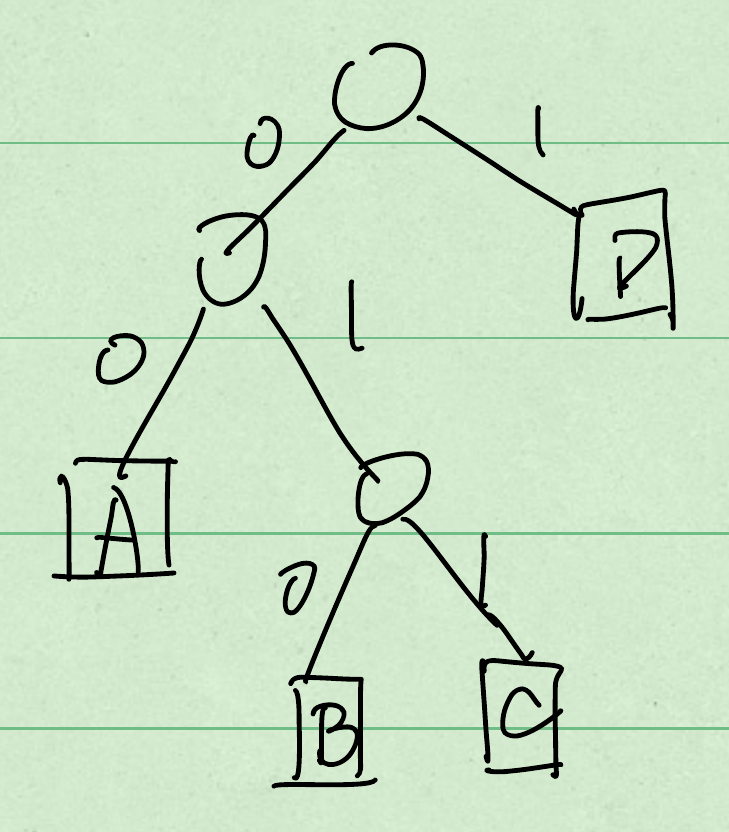
\includegraphics[width=0.3\textwidth]{binary-code-tree.png}
\end{figure}

Note that the symbols at the leaves are prefix code. The tree corresponding an optimal tree is a full binary tree, i.e. every internal node has two children. It is because if you have a internal node which is not full, then you are able to move everything below it one level up and reduce the code length.

Suppose we know the shape of the optimal tree which is a full binary tree.

\begin{claim}
	Any full binary tree has at least a pair of sibling leaves at the deepest leaves.
\end{claim}

\begin{claimproof}
	Choose one leaf $x$ at the deepest level. Its parent must have two children (say $x$ and $y$). $y$ cannot be internal node since $x$ is the deepest leaf. Therefore, $y$ must be the sibling leaf of $x$.
\end{claimproof}

\begin{claim}
	\textbf{Greedy Choice}: Pick the two symbols with least frequency and put them in the sibling leaves at the deepest level.
\end{claim}

\begin{claimproof}
	Prove the claim by exchange property. Suppose $x$ and $y$ are the two symbols of the least frequency. Suppose the sibling leaves at the deepest level have symbols $a$, $b$ and $\{a, b\} \neq \{x, y\}$.
	
	By exchanging the positions of a with $ x $ and $ b $ with $ y $, we can bring $ x, y $ to the deepest level. One can prove that this is no worst than the original tree.
	
\end{claimproof}

Make a new symbol $ xy $ in place of $ x $ and $ y $ so that $ f(xy) = f(x) + f(y) $. Suppose the length from root to $x$ is $ (d + 1) $. So the contribution of code length that $x$ and $y$ make is
\begin{align*}
	 & f(x) (d+1) + f(y)(d+1)\\
	=& (f(x) + f(y))(d+1)\\
	=& f(xy)(d+1)
\end{align*}
So the same tree with $xy$ made a symbol has cost that of $ f(xy) $ lower.

\subsection{Algorithm}
Combine two least frequent symbol $ x $ and $ y $ with one symbol $ xy $ with $ f(xy) = f(x) + f(y) $. 

Recursively solve the problem on the $ (n-1) $ symbols.